\documentclass[aspectratio=169,handout]{../latex_main/tntbeamer}  % you can pass all options of the beamer class, e.g., 'handout' or 'aspectratio=43'
\usepackage{dsfont}
\usepackage{bm}
\usepackage[english]{babel}
\usepackage[T1]{fontenc}
%\usepackage[utf8]{inputenc}
\usepackage{graphicx}
\graphicspath{ {./figures/} }
\usepackage{algorithm}
\usepackage[ruled,vlined,algo2e,linesnumbered]{algorithm2e}
\usepackage{hyperref}
\usepackage{booktabs}
\usepackage{mathtools}

\usepackage{amsmath,amssymb}

\DeclareMathOperator*{\argmax}{arg\,max}
\DeclareMathOperator*{\argmin}{arg\,min}

\usepackage{amsbsy}
\newcommand{\vect}[1]{\bm{#1}}
%\newcommand{\vect}[1]{\boldsymbol{#1}}

\usepackage{pgfplots}
\pgfplotsset{compat=1.16}
\usepackage{tikz}
\usetikzlibrary{trees} 
\usetikzlibrary{shapes.geometric}
\usetikzlibrary{positioning,shapes,shadows,arrows,calc,mindmap}
\usetikzlibrary{positioning,fadings,through}
\usetikzlibrary{decorations.pathreplacing}
\usetikzlibrary{intersections}
\pgfdeclarelayer{background}
\pgfdeclarelayer{foreground}
\pgfsetlayers{background,main,foreground}
\tikzstyle{activity}=[rectangle, draw=black, rounded corners, text centered, text width=8em]
\tikzstyle{data}=[rectangle, draw=black, text centered, text width=8em]
\tikzstyle{myarrow}=[->, thick, draw=black]

% Define the layers to draw the diagram
\pgfdeclarelayer{background}
\pgfdeclarelayer{foreground}
\pgfsetlayers{background,main,foreground}

% Requires XeLaTeX or LuaLaTeX
%\usepackage{unicode-math}

\usepackage{fontspec}
%\setsansfont{Arial}
\setsansfont{RotisSansSerifStd}[ 
Path=../latex_main/fonts/,
Extension = .otf,
UprightFont = *-Regular,  % or *-Light
BoldFont = *-ExtraBold,  % or *-Bold
ItalicFont = *-Italic
]
\setmonofont{Cascadia Mono}[
Scale=0.8
]

% scale factor adapted; mathrm font added (Benjamin Spitschan @TNT, 2021-06-01)
%\setmathfont[Scale=1.05]{Libertinus Math}
%\setmathrm[Scale=1.05]{Libertinus Math}

% other available math fonts are (not exhaustive)
% Latin Modern Math
% XITS Math
% Libertinus Math
% Asana Math
% Fira Math
% TeX Gyre Pagella Math
% TeX Gyre Bonum Math
% TeX Gyre Schola Math
% TeX Gyre Termes Math

% Literature References
\newcommand{\lit}[2]{\href{#2}{\footnotesize\color{black!60}[#1]}}

%%% Beamer Customization
%----------------------------------------------------------------------
% (Don't) Show sections in frame header. Options: 'sections', 'sections light', empty
\setbeamertemplate{headline}{empty}

% Add header logo for normal frames
\setheaderimage{
	% 
\includegraphics[height=\logoheight]{figures/TNT_darkv4.pdf}
	
\includegraphics[height=\logoheight]{../latex_main/figures/luh_logo_rgb_0_80_155.pdf}
	% 
\includegraphics[height=\logoheight]{figures/logo_tntluh.pdf}
}

% Header logo for title page
\settitleheaderimage{
	% 
\includegraphics[height=\logoheight]{figures/TNT_darkv4.pdf}
	
\includegraphics[height=\logoheight]{../latex_main/figures/luh_logo_rgb_0_80_155.pdf}
	% 
\includegraphics[height=\logoheight]{figures/logo_tntluh.pdf}
}

% Title page: tntdefault 
\setbeamertemplate{title page}[tntdefault]  % or luhstyle
% Add optional title image here
%\addtitlepageimagedefault{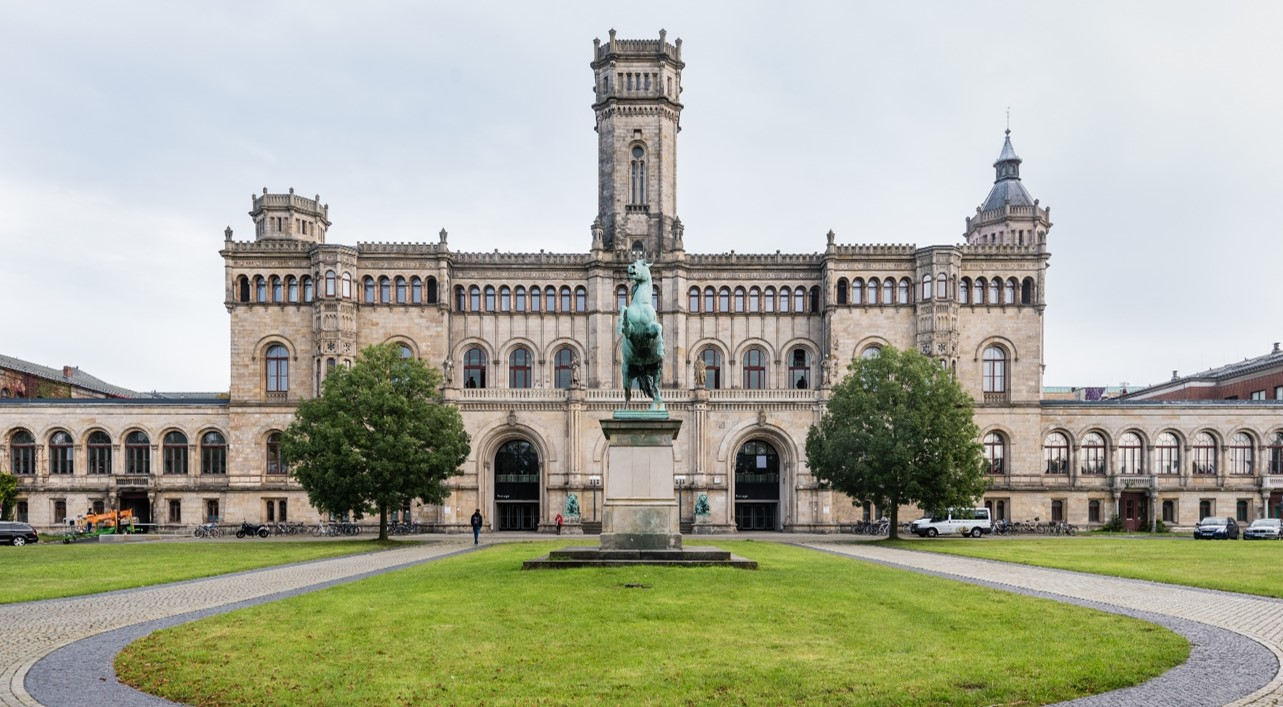
\includegraphics[width=0.65\textwidth]{figures/luh_default_presentation_title_image.jpg}}

% Title page: luhstyle
% \setbeamertemplate{title page}[luhstyle]
% % Add optional title image here
% \addtitlepageimage{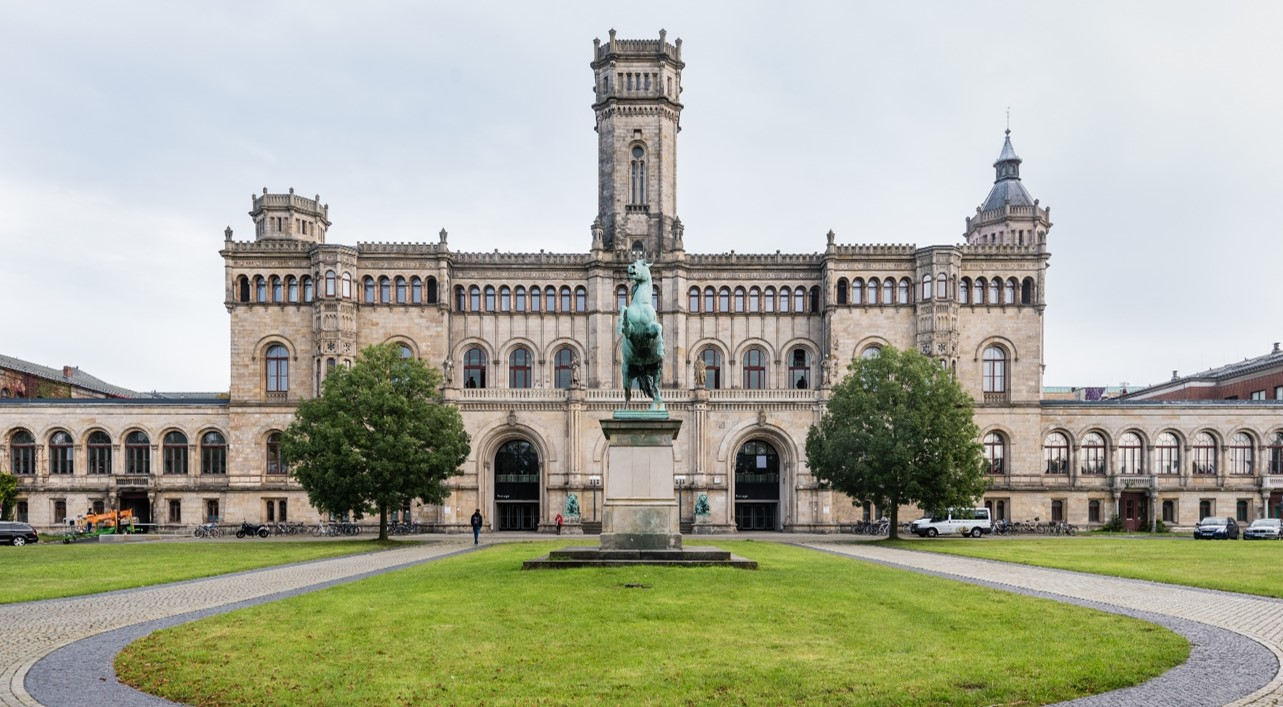
\includegraphics[width=0.75\textwidth]{figures/luh_default_presentation_title_image.jpg}}

\author[Abedjan \& Lindauer]{Ziawasch Abedjan \& Marius Lindauer\\[1em]
	
\includegraphics[height=\logoheight]{../latex_main/figures/luh_logo_rgb_0_80_155.pdf}\qquad
	
\includegraphics[height=\logoheight]{../latex_main/figures/DBIS_Kurzlogo.png}\qquad

\includegraphics[height=\logoheight]{../latex_main/figures/TNT_darkv4}\qquad

\includegraphics[height=\logoheight]{../latex_main/figures/L3S.jpg}	}
\date{Summer Term 2022; \hspace{0.5em} {
\includegraphics[height=1.5em]{../latex_main/figures/Cc-by-nc-sa_icon.svg.png}}; based on \href{https://ds100.org/fa21/}{[DS100]}
}


%%% Custom Packages
%----------------------------------------------------------------------
% Create dummy content
\usepackage{blindtext}

% Adds a frame with the current page layout. Just call \layout inside of a frame.
\usepackage{layout}


%%% Macros
%\renewcommand{\vec}[1]{\mathbf{#1}}
% \usepackage{bm}
%\let\vecb\bm

\title[Introduction]{Data Science Foundations}
\subtitle{Logistics of the Lecture}

%\institute{}


\begin{document}
	
	\maketitle

%----------------------------------------------------------------------
\begin{frame}[c]{Team}

\begin{columns}[T]




\column{0.2\textwidth}
\centering
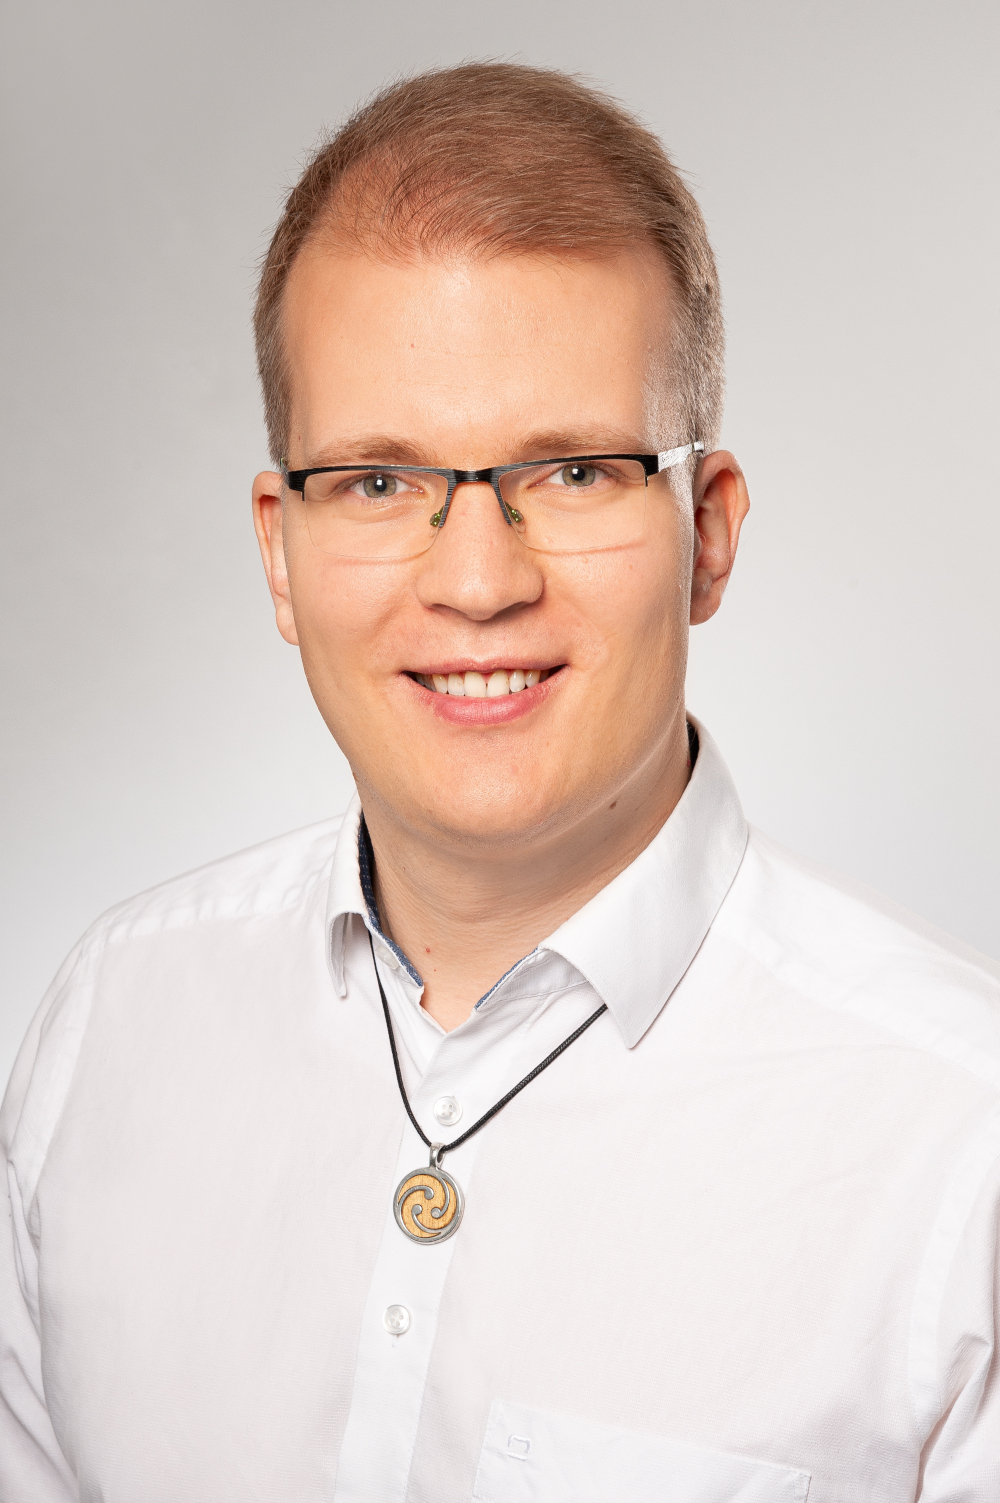
\includegraphics[height=8em]{./figures/Lindauer_Marius_004small.jpg}

Prof. Dr.\\ Marius Lindauer


\column{0.2\textwidth}
\centering
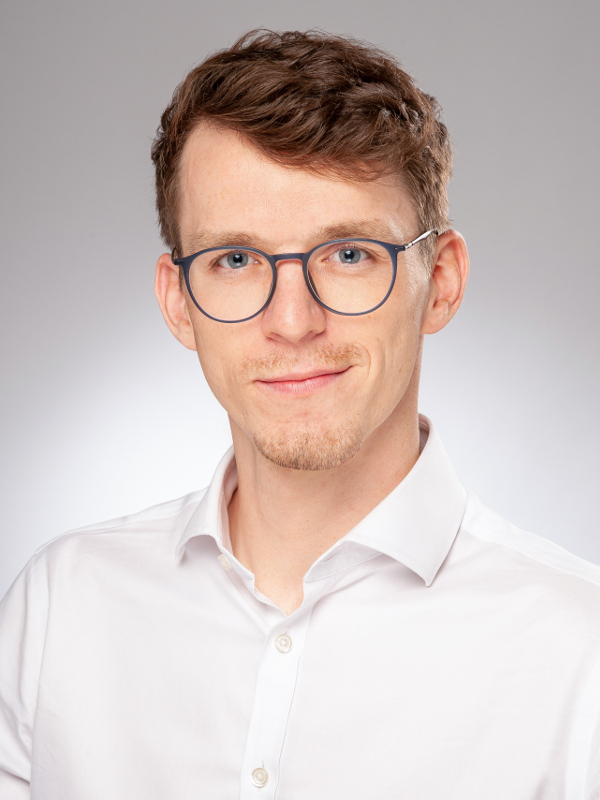
\includegraphics[height=8em]{./figures/tim}

Tim Ruhkopf\\

\end{columns}

\end{frame}
%----------------------------------------------------------------------


%-----------------------------------------------------------------------------------------------------------------------------
\begin{frame}[c]{Acknowledgments}

Large parts of the material (i.e. slides, figures and exercise) were created at \href{https://ds100.org/}{[Berkeley] (University of California)}. We thank them very much for allowing us to re-use their material.

\bigskip

\alert{Important}:
\begin{itemize}
    \item We changed material...
    \item We condensed it...
    \item We extended it...
    \item We fixed it...
\end{itemize}

\vspace{1em}

Prof. Ziawasch Abedjan contributed to the first two iterations of this course.

\end{frame}
%-----------------------------------------------------------------------


%-----------------------------------------------------------------------------------------------------------------------------
\begin{frame}[c]{Goals of the Lecture}

Data Science is not a spectator sport.
You will learn to code and to analyze!

You will be able to \ldots
\begin{enumerate}
  \item \alert{identify} steps needed to apply data science
  \pause
  \item \alert{explain} different data processing steps required in data science
  \pause
  \item \alert{choose} a promising combination of approaches to build data science pipelines
  \pause
  \item \alert{evaluate} data science pipelines on different datasets
  \pause
  \item \alert{visualize} data and results in data science
  \pause
  \item \alert{apply} data science to new tasks at hand
\end{enumerate}

\end{frame}
%-----------------------------------------------------------------------
%----------------------------------------------------------------------
\begin{frame}[c]{Course Overview}

\vspace*{-2em}
\begin{itemize} 
    \item Motivation
	\item Data Sampling and Probability 
        \item Visualization 
        \item Data Cleaning 
	\pause
	\item Intro to Modelling + Linear Regression 
	\item Learning Paradigms
	\item Classification 
        \item Deep Learning
        \pause
        \item Feature Engineering 	
        \item Bias and Variance + Data Reduction 
        \item Evaluation and AutoML 
	%\pause
	%\item Inference + Ethics 
	\pause
	\item Conclusion 
\end{itemize}

Optional video material on Inference and Ethics.


\end{frame}
%----------------------------------------------------------------------
%----------------------------------------------------------------------
\begin{frame}[c]{Course Format}

\begin{itemize}
	\item Concepts \& details
	\begin{itemize}
	  \item We provide sufficient details s.t. you can understand and use the techniques
	  \item We highly recommend that you dig deeper and read additional material to become a real expert
	\end{itemize}
	\smallskip
	\item Flipped-classroom lecture
	\begin{itemize}
        \item Watching video lectures at home
	  \item Discussion lecture (Wednesdays \alert{9am -10am})
        \item Guided lab exercise (Thursdays 11:00 - 12:30)
	\end{itemize}
	\smallskip
	\item Practical lab exercises and home works
	\begin{itemize}
	  \item implement it, use it and play with it!
	\end{itemize}
\end{itemize}

\end{frame}
%----------------------------------------------------------------------
%----------------------------------------------------------------------
\begin{frame}[c]{Learning Pyramid [\href{https://www.researchgate.net/publication/221801860_Applying_principles_from_Scientific_Foundations_for_Future_Physicians_to_teaching_chemistry_in_the_department_of_medicine_at_Chang_Gung_University}{Lou. 2012}]}

\centering
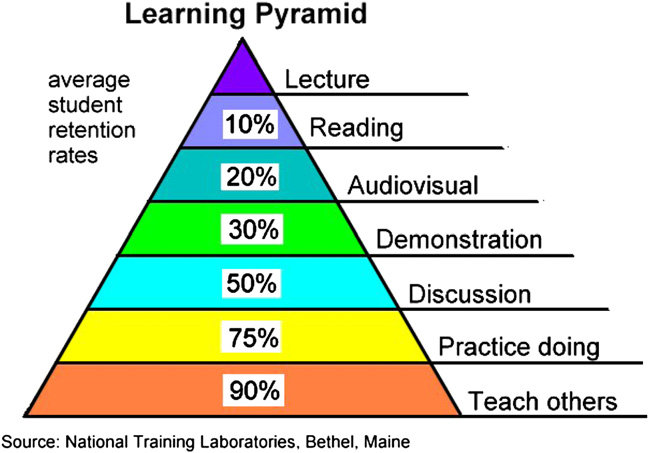
\includegraphics[width=0.6\textwidth]{figures/The-learning-pyramid-from-NTL-Institute-for-Applied-Behavioral-Science.jpg}

\end{frame}
%-----------------------------------------------------------------------
%----------------------------------------------------------------------
\begin{frame}[c]{Why Videos?}


\begin{itemize}
  \item Advantages of videos:
  \begin{itemize}
      \item Watch it whenever (\& wherever) you want
      \item Watch it at your own speed
      \begin{itemize}
          \item[$\leadsto$] Stop it if you need time to think about it
      \end{itemize}
      \item Go back and watch it again, if you missed or forgot something
      \item Annotate questions on the fly (e.g., using the Miro boards)
      \item After each video ($\sim$10-20min), you can take a break and\\ think about what you learned in this video (and whether you understood it)
      \item \alert{Recommendation:} Make your own notes while (or after) watching!
      \pause
      \item \alert{We have time in the lecture sessions to discuss the content!}
  \end{itemize}
  \medskip
  \pause
  \item Risks and challenges:
  \begin{itemize}
      \item You have to be self-disciplined 
      \item You have to wait with your questions until our meetings
      \begin{itemize}
          \item[$\leadsto$] Use the StudIP forum to discuss with your peers
          \item[$\leadsto$] ChatGPT? -- \alert{maybe} it will provide you a good explanation -- maybe it will hallucinate something
      \end{itemize}
  \end{itemize}
\end{itemize}

\end{frame}
%-----------------------------------------------------------------------

% %----------------------------------------------------------------------
% \begin{frame}[c]{Why Videos?}

% \begin{itemize}
%   \item Advantages of videos:
%   \begin{itemize}
%       \item Neither YOUTUBE nor NETFLIX VIDEOS!
%       \item Watch it whenever (wherever) you want
%       \item Watch it at your own speed
%       \begin{itemize}
%           \item[$\leadsto$] Stop it if you need time to think about it
%       \end{itemize}
%       \item Go back and watch it again, if you missed or forgot something
%       \item Annotate questions on the fly %(e.g., using the Miro boards)
%       \item After each video ($\sim$10-20min), you can take a break and\\ think about what you learned in this video (and whether you understood it)
%   \end{itemize}
%   \medskip
%   \pause
%   \item Risks and challenges:
%   \begin{itemize}
%       \item You have to be self-disciplined 
%       \item You have to wait with your questions until our meetings
%       \begin{itemize}
%           \item[$\leadsto$] Use our chat to discuss with your peers
%       \end{itemize}
%   \end{itemize}
% \end{itemize}

% \end{frame}
% %-----------------------------------------------------------------------
%----------------------------------------------------------------------
\begin{frame}[c]{Organization (Labs \& Homework)}

\vspace{-1em}
\begin{itemize}
  \item Every \alert{second} week new lab sheet
  \begin{itemize}
      \item Lab focus is aligned with lectures
      \item Check StudIP for exercise dates
      \item Do the lab exercise in the exercise sessions (Thursdays at 11:00am s.t.)
      \item Bring your own laptop
      %\item Watch videos and start to directly work on exercise 
      %\item[$\leadsto$] \alert{Deadline one day after the live session: Wednesday at 23:59}
  \end{itemize}
  \item Most exercises will be practical, i.e., you have to implement something
  \begin{itemize}
    \item Expected work load: 1.5h each week
  \end{itemize}
  \item Teamwork highly recommended, i.e., max team size of 3!
  \pause
  \item 1 mandatory homework
  \begin{itemize}
      \item $66\%$ of the points are required for passing the course 
      \item You'll get $5\%$ of bonus points for the exam, if you reach 90\% of the points\\
      \item Teamwork possible, max team size of 3
  \end{itemize}
  \pause
  \item Don't cheat (incl. plagiarism)
  \begin{itemize}
    \item Cheating: failing the course
  \end{itemize}
\end{itemize}

\end{frame}

\begin{frame}[c]{Organization (Labs \& Homework)}

\vspace{-1em}
\begin{itemize}
    \item To access the labs \& homework, you need to  \alert{register yourself TODAY after the lecture (!) on StudIP for the lecture}. 
    \item \alert{New accounts will be created ONLY on a weekly basis!}
    \item Make sure that the email address registered to your studip is ending with "uni-hannover.de".
    \item Tim Ruhkopf will send you an email with your credentials based on this list of participants. 
    \item Login using VPN (or on-site) and type  \href{https://jupyterhub.cluster.uni-hannover.de/} into your browser.
    \item Select the DataScience course in the dropdown and start a job 
    (this is an actual job on the LUIS Cluster, so waiting times might occur before resources are allocated to you.)
\end{itemize}

\end{frame}
%-----------------------------------------------------------------------
% %----------------------------------------------------------------------
% \begin{frame}[c]{Live Discussion}

% \begin{itemize}
%   \item Every week at Tuesday: 09:30am (s.t) - 11:30am\\ 
%   \item Room: Multimedia Room at L3S (15th floor, Appelstr. 9a)
%   \pause
%   \item Warning: Does not replace watching the recorded lecture videos!
%   \pause
%   \smallskip
%   \item Components:
%   \begin{enumerate}
%       \item You can ask anything related to the recent lecture videos or exercises
%       \item Break-out to discuss questions in small groups (if number of attendees to allow this)
%       \pause
%       \item Q\&A regarding the exercise
%       \pause
%       \item Interactive quiz where you can check whether you understood the main points
%   \end{enumerate}
%   \pause
%   \medskip
%   \item No recordings of the live sessions
% \end{itemize}

% \end{frame}
% %-----------------------------------------------------------------------
%----------------------------------------------------------------------
\begin{frame}[c]{Get in Touch with Us}

\begin{itemize}
  \item Lecture session every Wednesday (9am s.t.) and\\ exercise session (roughly) every second Thursday (11am s.t.)
  \item \alert{Use the forum in StudIP for all kinds of questions}
  \begin{itemize}
        \item[$\leadsto$] Contact Tim first if necessary 
      \item[$\leadsto$] Email to professor only in case of emergencies
  \end{itemize}
\end{itemize}

\end{frame}
%-----------------------------------------------------------------------
%----------------------------------------------------------------------
\begin{frame}[c]{Requirements for Attending}

\begin{itemize}
    \item Basics in \alert{Statistics} (mandatory)
    \begin{itemize}
        \item We will cover many concepts, but you need a basic understanding of the underlying math.
    \end{itemize}
  \item Programming in \alert{Python} (mandatory)
  \begin{itemize}
    \item All exercises will require that you implement something in~Python 
    \item We will show you the basics at the beginning in the exercises.\\ However if you never used Python before, it could get quite hard for you.
  \end{itemize}
  \item \alert{English} (mandatory)
    \begin{itemize}
    \item You can ask us any question also in German. However, we will reply in English.\\ So, you need to understand us ;-)
  \end{itemize}
\end{itemize}

\end{frame}
%-----------------------------------------------------------------------
%----------------------------------------------------------------------
\begin{frame}[c]{Final Exam}

\begin{itemize}
  \item Written Exam
  \item Show us that you understand the concepts
  \item Be a master of all the algorithms we showed you
  \item Be able to read and check code
  \item Be able to answer multiple-choice questions
  \item Fill blank-field text or graphics
  \item ...
\end{itemize}

\vspace{1em}
\alert{Date:} 20.08.2024, 8:00-10:00\\
\alert{Room:} 1101.E214

\end{frame}
%----------------------------------------------------------------------
%----------------------------------------------------------------------
\begin{frame}[c]{Additional Resources -- These are Hyperlinks!}

\begin{itemize} 
  \item Data science is such a big field
  \item Don't expect that you will learn everything in a single lecture / course\\ $\leadsto$ there might be parts you can only learn in our lecture (e.g., AutoML)
  \item There many awesome resources from which you can learn many more concepts
  \pause
  \bigskip
  \item Free online books
  \begin{itemize}
    \item \href{https://inferentialthinking.com/chapters/intro.html}{Inferential Thinking}
      \item \href{https://www.textbook.ds100.org/intro.html}{DS100 Textbook}
      \item Also see \href{https://www.ai.uni-hannover.de/en/studies/recommended-literature}{our institute website}
\end{itemize}
  \pause
  \item Online courses (MOOCs)
  \begin{itemize}
      \item \href{https://www.coursera.org/specializations/data-science-python}{Applied Data Science with Python Specialization} by the University of Michigan
      \item \href{https://www.coursera.org/learn/machine-learning/home/welcome}{Machine Learning} by Andrew NG
  \end{itemize}
  \pause
  \item \href{https://www.kaggle.com/}{Kaggle} for online competitions, datasets and code
  \begin{itemize}
      \item If you can become a grant master at Kaggle, you have very good chances for job offers
      \item Participate in competitions, look for help in forums, polish your skills!
  \end{itemize}
\end{itemize}

\end{frame}
%----------------------------------------------------------------------
%----------------------------------------------------------------------
\begin{frame}[c]{Opportunities and Risks}

``Data Science Foundations'' is a basic lecture.

\bigskip
\pause

Opportunities:
\begin{itemize}
  \item Get all the basics you need to do your own first data science projects
  \item Perfect foundation for other AI courses at the LUH (most of them in the masters; see next slide)
\end{itemize}

\medskip

Risks:
\begin{itemize}
  \item You will find some typos and issues in the slides;\\ please tell us if you find something
  \item We will not cover the newest DL methods
\end{itemize}

\medskip
$\to$ Give us some feedback and we will improve the course!

\end{frame}
%-----------------------------------------------------------------------
%----------------------------------------------------------------------
\begin{frame}[c]{AI@LUH}

\vspace{-2em}
\centering
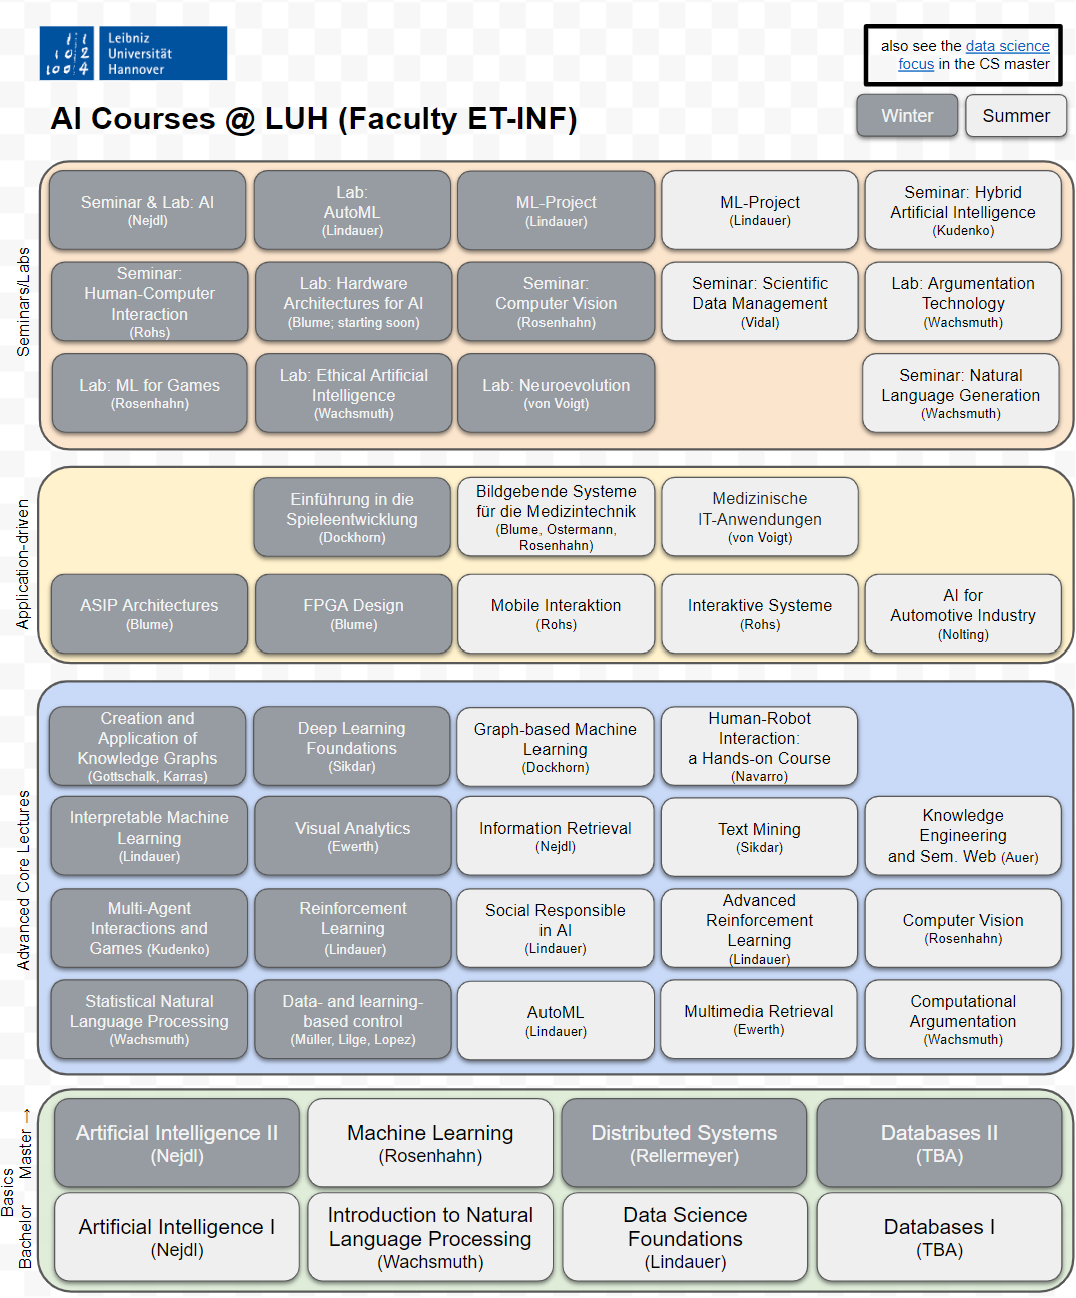
\includegraphics[width=0.43\textwidth]{figures/AI_Courses_LUH}

\end{frame}
%----------------------------------------------------------------------
%----------------------------------------------------------------------
\begin{frame}[c]{Leibniz AI Academy}

\centering
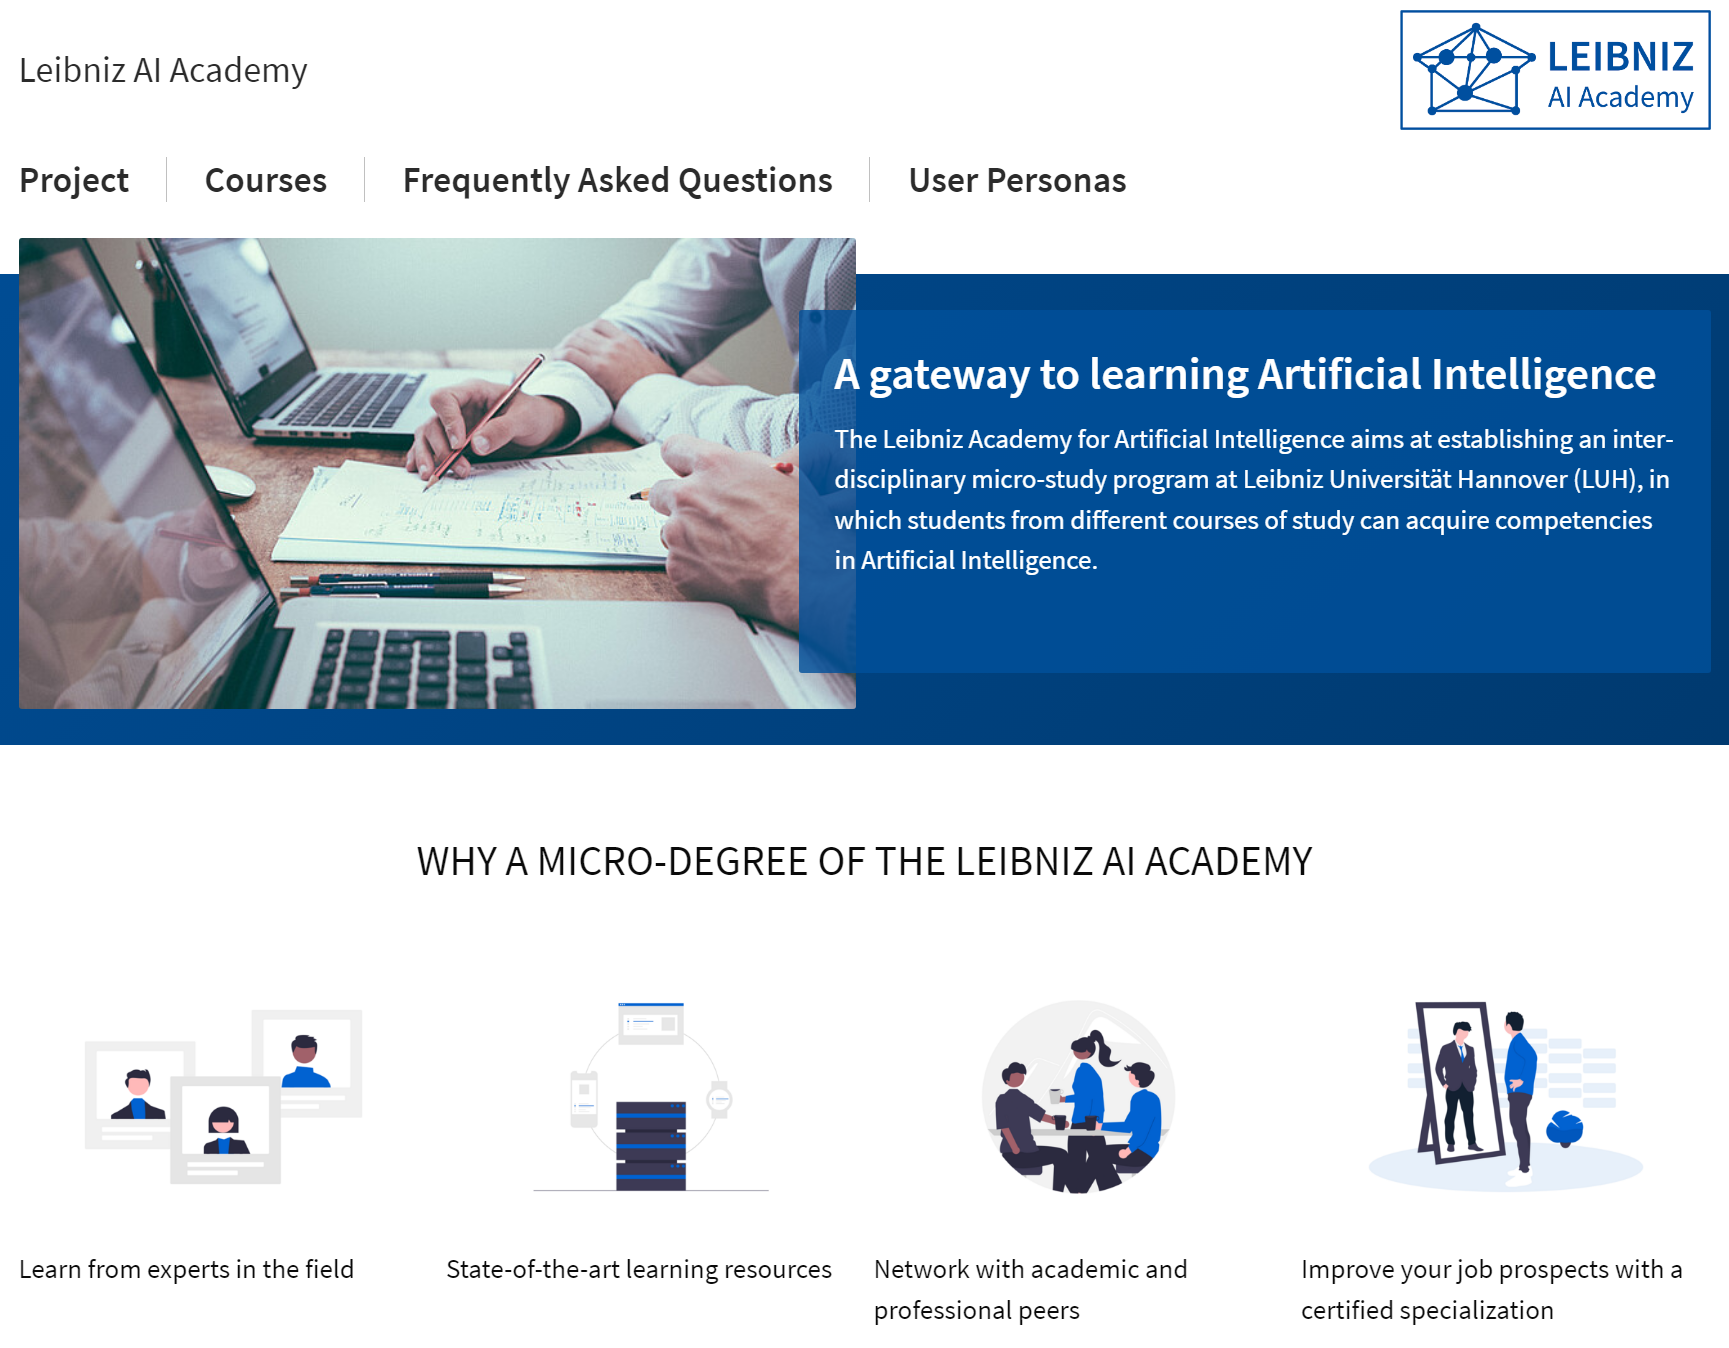
\includegraphics[width=0.6\textwidth]{figures/leibniz_ai_academy.png}

\end{frame}
%----------------------------------------------------------------------
%----------------------------------------------------------------------
\begin{frame}[c]{DS Lecture as Part of Leibniz AI Academy}

\centering
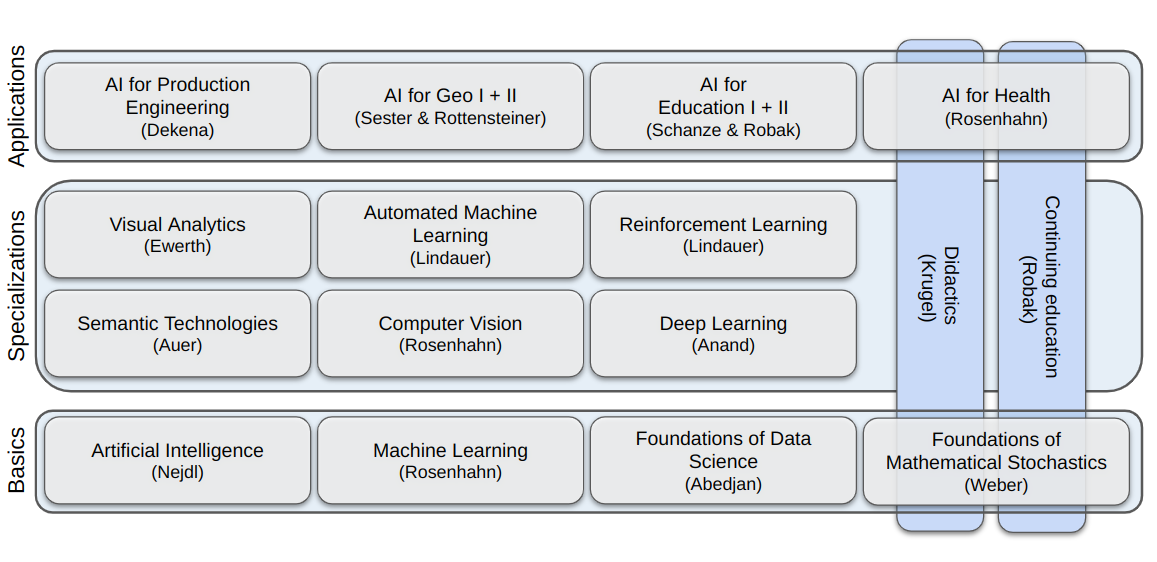
\includegraphics[width=0.8\textwidth]{figures/LAI-New-Blue.png}

\end{frame}
%----------------------------------------------------------------------%----------------------------------------------------------------------
\begin{frame}[c]{Introduce yourself}


\begin{center}
\huge
    Introduce yourself!
\end{center}

\begin{itemize}
    \item What drives you to be here?
    \item What interests you in data science?
    \item Do you already have hands-on experience in data science?
    \item Are you looking for team members for exercises and home work?
\end{itemize}

\end{frame}
%-----------------------------------------------------------------------

% \end{frame}

\begin{frame}[c]{}

\centering
\huge
Questions?

\end{frame}

	
\end{document}
